\chapter{Magnetic particle separation simulation}\label{ch:magneticParticleSeparationSimulation}

%\textit{To investigate particle movement and separation mechanisms in microfluidic channels, the computational simulation approach offers cost and turnaround time benefits, since it allows to explore and possibly eliminate numerous preliminary designs. In result, the manufacturing and testing of a host of competing microchannels or processes can be partially replaced with modelling. Moreover, the detail and specificity that simulation offers can help explore the exact trajectory of magnetic particle in any given magnetic field.}

\section{Introduction}
Magnetic particles can be manipulated using an external magnetic field, independently from the motion of the surrounding liquid, which is known as magnetophoresis (see Chapter~\ref{ch:magnetophoresis}). The manipulation of these magnetic particles allows for particle sorting or particle separation. 

In this work, the magnetic particles and the effect of an external magnetic field on their trajectory will be simulated using the Lagrangian tracking scheme. Due to the assumed low particle concentration and small particle size, where interparticle forces can be neglected and one-way coupling can be assumed, the Lagrangian approach is the more accurate method, because it allows to simulate individual particle trajectories. 

The simulation was modelled in two steps. The first step was the steady state modelling of the magnetic force using the commercially available FEM software package ANSYS Maxwell and under consideration of all aforementioned numerical simulation techniques. The simulation results were exported to a uniform mesh, which could be stored in an array in which the position of the array represents the location of the magnetic field result of a specific element. 

In a second step single particle trajectories were simulated by importing the magnetic field results into Matlab. Through a postanalysis algorithm the magnetophoretic driving force could be calculated at every single node of the imported array. Since the magnetophoretic driving force of the specific magnet configuration is calculated, rather than the magnetic force on a single particle, the simulation retains the flexibility to simulate different magnetic particle properties. The magnetic force on a magnetic particle can then be calculated by simply multiplying the magnetophoretic driving force with the particle's magnetophoretic mobility, which can either be obtained theoretically or experimentally. 

This modelling technique allows the analysis of the effects of varying magnet configuration, particle characteristics and fluidchannel geometry on the magnetic separation process.

\section{Lagrangian particle tracking}\label{sec:lagrangianParticleTracking}
The Lagrangian approach for the simulation of the disperse phase is based on Newton's equation of motion. The equation of motion for small rigid spheres was proposed by Maxey and Riley~\cite{Maxey1983}.

Efficient algorithms for Lagrangian particle tracking in fluid flow are an ongoing research topic. To date a number of algorithms have been implemented in discrete particle simulations. The reader can refer to~\cite{Gouesbet1999,Lain2002,Stuart2011} for the historical development of such algorithms.

The Lagrangian tracking scheme maps the particle positions at discrete time steps and can be given by: 

\begin{equation}
	\mathbf{x}(t+\delta t) = \mathbf{x}(t)+\mathbf{u}_{p}\delta t
	\label{eqn:lagrangianEquation}
\end{equation}

in which $\mathbf{x}(t)$ is the location vector of the fluid particle at time $t$, $\mathbf{u}_{p}$ is the instantaneous particle velocity vector and $\delta t$ is an incremental time step, small enough so that the particle velocity vector $\mathbf{u}_{p}$ is essentially constant during the finite time step $\delta t$.

%The particle velocity vector $\mathbf{u}_{p}$ has only two non-zero components because gravity was neglected: 
%\begin{equation}
%	\mathbf{u}_{p} = 	\begin{bmatrix}
%       						u_{px} \\
%       						0 \\
%       						u_{pz}
%     					\end{bmatrix}
%\end{equation}
%where $u_{px}$ and $u_{pz}$ are the velocity components in $x$ and $z$ direction respectively. 

%Since the magnetic force acts perpendicular to the flow direction, the velocity vector components can be treated separately. The calculation of the velocity component in $z$ direction is straight forward, because the particle is assumed to be small enough such that it always has the same velocity as its surrounding fluid and also follows the streamlines perfectly. The fluid velocity profile in a rectangular duct is well documented in the literature and an analytically solution can be found as also shown previously~\cite{White2006}. 

%A bigger challenge is the efficient calculation of the magnetically induced particle velocity at every possible particle position in the $x-y$ plane. This task requires two actions: firstly, to find the closest grid node to the current particle position and secondly to interpolate the magnetopohretic velocity across adjacent nodes to find the exact magnetophoretic velocity. The pre-limitation of the magnetophoretic velocity is an essential step to increase computing efficiency. 

The efficient calculation of the magnetically induced particle velocity at every possible particle position is challenging. This task requires two actions: firstly, to find the closest grid node to the current particle position and secondly to interpolate and smooth the magnetopohretic velocity across adjacent nodes to find the exact magnetophoretic velocity. The pre-conditioning of the magnetophoretic velocity matrix is an essential step to increase computing efficiency. 

As can be seen from Equation~\ref{eqn:lagrangianEquation} the simulation of single magnetic particle movement under the influence of an applied magnetic field in a channel flow develops to be a transient problem. This means that time needs be taken into account. Thus, the accuracy of this approach depends not only on the computational magnetic field solution, but also on the chosen discrete time step $\delta t$. Therefore, the size of the time step in the Lagrangian time marching method requires some consideration. An obvious approach to address accuracy is to reduce the time step, resulting in reducing the error, but it is also not possible to decrease time step infinitely due to computational affordability. The condition which needs to be met to guarantee accuracy and computational stability is the Courant-Friedrichs-Lewy (CFL) condition~\cite{Courant1967}. 

\begin{equation}
	\frac{\mathbf{u}_{p}^{i}\delta t}{\omega} \leq 1
	\label{eqn:courantFriedrichsLewy} 
\end{equation}

where $\mathbf{u}_{p}^{i}$, $\delta t$ and $\omega$ are the velocity vector of the $i^{\text{th}}$ particle, the time marching step and the grid size $\omega$, respectively. In this work the grid length $\omega$ is in the order of a couple of tens of $\mu$m ($10^{-5} \text{m}$) in the region of where the fluid channel is located, while the maximum mean particle velocity used is $\bar{u}_{p}\approx 8.3 \text{mm/s}$. Thus the simulation time step should be $\delta t \approx 1 \text{ms}$ in order to meet the CFL condition.

\section{Particle trajectory simulation}\label{sec:particleTrajectorySimualation}
Based on the numerically simulated magnetophoretic force fields of the two magnet configurations, double magnet configuration and quadrupole magnet configuration, particle trajectories have been simulated in order to work out the particle separation efficiency of the two magnet designs in a continuous or pulse mode manner. 

The simulation follows the heuristic approach of all properties pertaining to materials are constant, as it is discussed by Melcher~\cite{Melcher1981}. This means the parameters have no magnetic field dependence, and the experimentally found mean magnetophoretic mobilities (Chapter~\ref{ch:magnetophoresis}) can be used. Chapter~\ref{ch:magnetophoresis} has shown that this approach is only an approximation and thus further simulations might be needed. 

The separation efficiency of the magnet configurations was tested by using a Monte Carlo method. In order to get statistical significance at least $400$ particle trajectories were sampled in each simulation. The sample size was estimated by using a maximum variance scheme where an underlying binomial distribution of the outcome was assumed and a confidence interval of $95\%$ was used~\cite{Kreyszig2006}. 

At the inflow particles were randomly distributed (uniform distribution) across one of the inlet's cross-section and were released in a region where the magnetic force on a single particle has dropped to $10\%$ of its maximum possible value the particles will experience within the fluidchannel. This occurs at a distance $6$ mm away from the magnet configuration. 

As they travel along the channel the magnetic force starts acting on them. The magnetic force pushes or pulls the particles towards the gathering points. The computer simulates the particles until they either settled at the channel walls or travelled through the whole length of the channel. The sampling time step was set to $1$ millisecond, as previously determined. 

The performance of the separation device is determined by its collection efficiency $\zeta$, which can either be formulated in absolute or relative terms. The absolute separation efficiency, $\zeta_{a}$, is defined by the fraction of magnetic particles that enter the separation channel and leave the channel through the designated exit, whereas the relative separation efficiency, $\zeta_{r}$, only takes the ratio of the number of particles exiting the designated channel over the number of particles coming out of the system. Both efficiency ratios will be used here and can be mathematically expressed as follows:

\begin{eqnarray}
	\zeta_{a} = \frac{N_{out}^{k}}{N_{in}}\\
	\zeta_{r} = \frac{N_{out}^{k}}{N_{out}}
	\label{eqn:separationEfficiency}
\end{eqnarray}

where $N_{in}$ and $N_{out}$ are the total number of particles going in and coming out of the system, respectively and $N_{out}^{k}$ is the number of particles leaving the designated exit $k$.

%where $N_{out}^{i}$ is the number of particles leaving the designated exit $i$, $N_{out}$ is the number of particles coming out of the system and $N_{in}$ is the total number of particles initially fed into the system.

The collection efficiency is expected to depend on the mean flow velocity and the applied external magnetic field. In order to investigate both effects, two series of numerical simulations have been performed, namely \textit{continuous} and \textit{pulse} mode separation.

%%%%%%%%%%%%%%%%%%%%%%%%%%%%%%%%%%%%%%%%%%%%%%%%%
%%%%%%%%%%%%%%%%%%%%%%%%%%%%%%%%%%%%%%%%%%%%%%%%%
%%%%%%%%%%%%%%%%%%%%%%%%%%%%%%%%%%%%%%%%%%%%%%%%%
%\subsection{Flow rate consideration}\label{subsubsec:flowRateConsideration}
%The relative separation efficiency $\zeta_{r}$ in continuous flow depends on the total interaction time one magnetic particle has with the applied magnetic field. Thus, $\zeta_{r}$ will be a function of the mean flow velocity in the main channel, because the particle interaction time can be controlled by the flow rate.
%
%The examined particles have a magnetophoretic mobility between $1.7-7.9 \times 10^{-11}$ $\text{m}^3/\text{T}\cdot\text{A}\cdot\text{s}$. Particles with higher magnetophoretic mobility will move further in any given time interval than particles with a lower magnetophoretic mobility. Therefore, the flow rates need to be adjusted based on the particle type used. 
%
%In the double magnet configuration the particles are fed through the center channel. In the worst case, particles need to travel across a distance of maximum $1$ mm before they are considered to be separated from the sample flow. At the same time, particles can at most move half of the channel's height ($200$ $\mu$m) before they hit the top or bottom, respectively. By knowing the mean magnetophoretic driving force one can work out the time needed to move particles over a certain distance in horizontal and/or vertical direction.
%
%The ANSYS Maxwell simulations gave a mean magnetophoretic driving force in horizontal and vertical directions of $|S_{\parallel}|=9.1\times10^{5}$ T$\cdot$A/m$^{2}$ and $|S_{\bot}|=5.1\times10^{4}$ T$\cdot$A/m$^{2}$, respectively. The mean magnetophoretic driving force is taken across the cross-section of the center inlet channel and over a magnet length in $z$ direction of $18$ mm. 
%
%The mean magnetically induced velocity of the different tested particles and their minimum time needed to travel over the whole width of the inlet channel ($1$ mm) in horizontal direction on a conservative distance of only one quarter of the channel height ($0.1$ mm) and the corresponding flow rates are given in Table~\ref{tab:particleMigrationTime}
%
%% mobilities have changed 
%\begin{table}[htb]
%\begin{center}
%\caption[Particle mean migration time in horizontal and vertical direction]{Particle mean migration time in horizontal and vertical direction.}\vspace{1ex}
%\label{tab:particleMigrationTime}
%\begin{tabular}{lccccrc}
%\hline
%Particle type & $\nu_{p}$ & $\bar{u}_{\parallel}$ & $t_{\parallel}$ & $\bar{u}_{\bot}$ & $t_{\bot}$  & $\dot{Q}_{min}$ \\ 
%& [mm$^3$/T$\cdot$A$\cdot$s] & [$\mu$m/s] & [s] & [$\mu$m/s] & [s] & [$\mu$l/min] \\
%\hline
%ScreenMAG 	& 0.0168 & 13.6 & 74 & 0.8 & 125 	& 17.5 \\
%SiMAG 		& 0.0585 & 14.0 & 72 & 0.8 & 125 	& 18.0 \\
%MyOne 		& 0.0201 & 21.3 & 50 & 1.2 & 84 	& 25.9 \\
%M280		& 0.0536 & 46.2 & 22 & 2.6 & 39 	& 58.9 \\
%M270		& 0.0787 & 70.8 & 15 & 4.0 & 25 	& 86.4 \\ 
%\hline
%\end{tabular}
%\end{center}
%\end{table}
%
%The double magnet configuration has a length of $20$ mm, which is the maximum distance the particle can possibly interact with the magnetic field. Since the gathering points vanish around the corner of the magnets (at $z=\pm 10$ mm), a maximum interaction distance of only $18$ mm will be considered here. Given the minimum time to separate the particles, a minimum flow rate, $\dot{Q}_{min}$, can be computed to give the  particles enough time to migrate towards the sheath flow (see Table~\ref{tab:particleMigrationTime}). 
%
%Particles that reach the end of the magnetically exposed channel, without colliding with the inner wall, still need to exit the magnetic field and flow out through the designated outlets. In order to understand the effects the edges of the magnets may have on the trajectories of the particles when they try to leave magnetic field, a very conservative model was used. Rather than having the particles moving along the side of the magnet configuration, it is assumed the particle laden flow runs in the center plane ($y=0$) through the centre of the magnetic configuration, as shown in Figure~\ref{fig:magneticForceWhenExitingScheme}. 
%
%\begin{figure}[htb]
%\centering
%\includegraphics[width=0.75\textwidth]{img/chapters/magneticSeparation/velocityConsideration.PNG}
%\caption[Schematic for flow rate consideration]{Schematic for flow rate consideration. Conservative approach is taken where a particle is assumed to move along the $z$ through the center of a double magnet configuration.}
%\label{fig:magneticForceWhenExitingScheme}
%\end{figure}
%
%The results show that a flow rate of at least $16.4$ $\mu$l/min for particles with a magnetophoretic mobility of $0.0149$ $\text{mm}^3/\text{T}\cdot\text{A}\cdot\text{s}$ and for particles with a magnetophoretic mobility of $0.0695$ $\text{mm}^3/\text{T}\cdot\text{A}\cdot\text{s}$ a minimum flow rate of $85.5$ $\mu$l/min is necessary to generate enough drag force to make the particles exiting the area between the magnets. Since the minimum velocities to make the particles leaving the applied magnetic field is always smaller for all particle types than the lower limit for the particles to have enough time to get separated, trapping at the end of the fluid channel should not be an issue. 
%
%Unfortunately, this quick analysis only gives a rough estimation about the needed flow rates, because neither the magnetic force on the particles, nor the fluid velocity in the channel are constants. But the results serve as a guideline.
%%%%%%%%%%%%%%%%%%%%%%%%%%%%%%%%%%%%%%%%%%%%%%%%%
%%%%%%%%%%%%%%%%%%%%%%%%%%%%%%%%%%%%%%%%%%%%%%%%%
%%%%%%%%%%%%%%%%%%%%%%%%%%%%%%%%%%%%%%%%%%%%%%%%%

\section{Particle trajectory simulation in continuous flow}\label{sec:particleTrajectorySimulationInContinuousFlow}

\subsection{Single particle trajectory}
\label{subsec:singleParticleTrajectory}
The continuous separation efficiency of the double magnet configuration was evaluated by simulating single particle trajectories. The particles were introduced through the center inlet of the iBidi channel with an aspect ratio of $1$ between all flow rates. Due to the symmetry of the separation setup, only the upper half of the device needed to be simulated, as depicted in Figure~\ref{fig:particleIntroductionSchemeDoubleMagnetConfiguration}. 

\begin{figure}[htb]
        \centering
        \begin{subfigure}[b]{0.45\textwidth}
                \includegraphics[width=\textwidth]{img/chapters/magneticSeparation/particleInletHydrodynamicFocusingScheme.PNG}
                \caption{}  
        \end{subfigure}
        \begin{subfigure}[b]{0.45\textwidth}
                \includegraphics[width=\textwidth]{img/chapters/magneticSeparation/particleInletCrosssectionScheme.PNG}
                \caption{}                
        \end{subfigure}
        \caption[Schematic where particle are introduced in the continuous flow simulation]{Schematic where particle are introduced in the continuous flow simulation. The grey area indicates particle laden solution. (a) Top view: Particles are released through the center channel of the separation device. (b) Cross sectional view: Particles are randomly distributed across the top half of the centre channel due to symmetry. Sketches are not to scale.}
        \label{fig:particleIntroductionSchemeDoubleMagnetConfiguration}
\end{figure}

For the simulation the optimal vertical magnet gap of $2.64$ mm was chosen and the center of the double magnet configuration was placed $4.6$ mm away from the channel side wall, such that the gathering points align within the fluid channel but $0.5$ mm away from the channel's side wall pointing to one of the sheath flow exits.

Figure~\ref{fig:relativeSeparationEfficiencyAndParticleThroughputDoubleMagnetConfiguration} shows the simulated relative separation efficiency and particle throughput of the double magnet configuration for various flow rates, ranging from $10-375$ $\mu$l/min. The magnetophoretic mobility was set to $5.85 \times 10^{-11}$ m$^{3}$/T$\cdot$A$\cdot$s and  $2.01 \times 10^{-11}$ m$^{3}$/T$\cdot$A$\cdot$s which are the equivalent values of the experimentally determined magnetophoretic mobility for the $1$ $\mu$m sized SiMAG (Chemicell) and MyOne (Dynabeads) particles in water. 

\begin{figure}[htb]
        \centering
        \begin{subfigure}[b]{0.48\textwidth}
                \includegraphics[width=\textwidth]{img/chapters/magneticSeparation/relativeSeparationEfficiencyDoubleMagnetConfigurationSiMAGandMyOne2.eps}
                \caption{}  
        \end{subfigure}
        \begin{subfigure}[b]{0.48\textwidth}
                \includegraphics[width=\textwidth]{img/chapters/magneticSeparation/throughputDoubleMagnetConfigurationSiMAGandMyOne2.eps}
                \caption{}                
        \end{subfigure}
        \caption[Relative magnetic separation efficiency and particle throughput of two different particles types for different flow rates using the double magnet configuration]{(a) Relative magnetic separation efficiency and (b) particle throughput for flow rates ranging between $6 - 375$ $\mu$l/min in the main channel. Particles which have crossed the $x=-0.5$ mm line without colliding with any surface are considered to be separated. The particle properties are set to the $1$ $\mu$m sized SiMAG-Silanol (Chemicell) and MyOne (Dynabeads) particles.}
        \label{fig:relativeSeparationEfficiencyAndParticleThroughputDoubleMagnetConfiguration}
\end{figure}

In order for the particles to be considered to be separated, they did not have to reach their final gathering position, but needed to move horizontally across into the streamlines of the sheath flow ($x=-0.5$ mm) and must have reached the end of the fluid channel. 

It can be clearly seen (Figure~\ref{fig:relativeSeparationEfficiencyAndParticleThroughputDoubleMagnetConfiguration}) that the relative separation efficiency and the particle throughput are inversely proportional. Also the increase in magnetophoretic mobility positively effects the relative separation efficiency, but comes with the price of a reduced particle throughput. There is a trade-off between the relative separation efficiency and the particle throughput. At a relative separation efficiency of $100\%$ only up to $10\%$ of the introduced particles can be collected at the designated exit channel, which means most particles are getting stuck in the system. This result was also experimentally observed at a flow rate of $3$ $\mu$l/min, when nearly all particles were trapped in the device. Therefore, a sufficiently high flow rate is needed to guarantee a viable throughput. 

The particles also experience a force in $z$ direction, which hinders the particles from leaving the magnetic impact zone. A minimum flow rate of $2$ $\mu$l/min is necessary to generate enough drag force to push every particle type out of the magnetic field. Hence, the magnetic force cannot be the limiting factor for the low particle throughput.

In order to provide clarity of what exactly happens to the particles while moving along the separation device their individual trajectories have been computed. Figure~\ref{fig:scatterPlotDoubleMagnetConfiguration} shows the initial and final position of the magnetic particles across the fluid channel's cross-section, after their trajectory simulation has terminated. As mentioned, only the top half of the fluid channel ($|y| \leq 0.2]$ mm) is simulated. The different colours used here show particles which reached the end of the fluid channel and were successfully separated (green), reached the end of the channel but did not get separated (blue), get successfully separated but get stuck at the top of the channel surface (orange) or did not get separated and get stuck (red).

\begin{figure}[htb]
        \centering
        \begin{subfigure}[b]{0.48\textwidth}
                \includegraphics[width=\textwidth]{img/chapters/magneticSeparation/scatterPlotDoubleMagnetConfiguration_6ulmin_color.eps} % _color
                \caption{}  
        \end{subfigure}
        \begin{subfigure}[b]{0.48\textwidth}
                \includegraphics[width=\textwidth]{img/chapters/magneticSeparation/scatterPlotDoubleMagnetConfiguration_15ulmin_color.eps} % _color
                \caption{}                
        \end{subfigure}
        \begin{subfigure}[b]{0.48\textwidth}
                \includegraphics[width=\textwidth]{img/chapters/magneticSeparation/scatterPlotDoubleMagnetConfiguration_50ulmin_color.eps} % _color
                \caption{}                
        \end{subfigure}
        \begin{subfigure}[b]{0.48\textwidth}
                \includegraphics[width=\textwidth]{img/chapters/magneticSeparation/scatterPlotDoubleMagnetConfiguration_100ulmin_color.eps} % _color
                \caption{}                
        \end{subfigure}
        \caption[Scatter plot of particles' initial starting end end position for different flow rates using the double magnet configuration]{Scatter plot of the particles' initial starting and end position for different flow rates ranging from (a) $6$ $\mu$l/min (b) $15$ $\mu$l/min (c) $50$ $\mu$l/min (d) $100$ $\mu$l/min. The open circles represent the starting position and the filled circles show their final position. Particles have a magnetophoretic mobility of $1.54 \times 10^{-11}$ m$^3$/T$\cdot$A$\cdot$s which is the value experimentally found for Chemicell's SiMAG-Silanol particle.}
        \label{fig:scatterPlotDoubleMagnetConfiguration}
\end{figure}

By looking at Figure~\ref{fig:scatterPlotDoubleMagnetConfiguration} it becomes evident that only a limited number of particles get actually separated. Only particles released at specific positions across the inlet (green circles) get drawn into the buffer flow without hitting the surface. This forms a unique particle release pattern across the inlet cross section for the different flow rates.

However, the majority of the particles get trapped at the top of the fluid channel. The vertical force makes the particles migrate to the top, where the fluid velocity essentially drops to zero due to the no slip boundary conditions at any surface. Thus, particles which hit a surface of the device do no longer move forwards and will be deemed as \textit{lost}, as they are difficult to recover using continuous flow at low flow rates. This phenomena is also represented in the simulation algorithm by stopping the corresponding particle trajectory. Therefore, particle interaction with a solid wall might also need to be considered.

\subsection{Particle trajectories of agglomerates}
\label{subsec:particleTrajectoriesOfAgglomerates}
As soon as superparamagnetic particles are exposed to a magnetic field, they become magnetized and start attracting other particles in their close vicinity. This causes particle to form agglomerates as it could be observed in the magnetophoretic study for magnetic particle agglomerates (see Chapter~\ref{ch:magnetophoresis}).

Even when starting from a fully suspended solution at low concentration ($10^{-6}$ particles per millilitre), one cannot guarantee that no particle agglomerates will be formed. Particle-particle interaction can also occur at low concentration while particles travel through the device and happen to be close enough. Therefore, particle trajectories of particle clusters should also be studied. 
 
The particle agglomerate model presented here shows that the drag force on a cluster of particles does not increase linearly, but its magnetic force does. This model is implemented in the simulation. Particle agglomerations of up to $5$ particles are studied here. Figure~\ref{fig:relativeSeparationEfficiencyAndParticleThroughputDoubleMagnetConfigurationAgglomerations} shows the relative separation efficiency $\zeta$ and the particle throughput for different used flow rates.

\begin{figure}[htb]
        \centering
        \begin{subfigure}[b]{0.48\textwidth}
                \includegraphics[width=\textwidth]{img/chapters/magneticSeparation/relativeSeparationEfficiencyDoubleMagnetConfiguration_agglomerations.eps}
                \caption{}  
                \label{fig:relativeSeparationEfficiencyDoubleMagnetConfigurationAgglomerations}
        \end{subfigure}
        \begin{subfigure}[b]{0.48\textwidth}
                \includegraphics[width=\textwidth]{img/chapters/magneticSeparation/throughputDoubleMagnetConfiguration_agglomerations.eps}
                \caption{}       
                \label{fig:particleThroughputDoubleMagnetConfigurationAgglomerations}         
        \end{subfigure}
        \caption[Relative magnetic separation efficiency and particle throughput of particle agglomerates for different flow rates using the double magnet configuration]{(a) Relative magnetic separation efficiency and (b) particle throughput for flow rates ranging between $30 - 375$ $\mu$l/min in the main channel. Particles which have crossed the $x=-0.5$ mm line without colliding with any surface are considered to be separated. The particle properties for a single particle are set equal to the properties of a $1$ $\mu$m sized SiMAG-Silanol (Chemicell) particle.}
        \label{fig:relativeSeparationEfficiencyAndParticleThroughputDoubleMagnetConfigurationAgglomerations}
\end{figure}

Because of the saturating drag force with an increasing number of particles in an agglomeration, larger clusters experience a larger magnetophoretic drift velocity than agglomerations which contain fewer particles. This causes larger particle agglomerations to respond more quickly to the applied magnetic field, which explains the increasing relative separation efficiency (Figure~\ref{fig:relativeSeparationEfficiencyDoubleMagnetConfigurationAgglomerations}). Unfortunately, the increased magnetically induced velocity also causes larger cluster to get stuck at the inner surface of the fluid channel which leads to a lower overall particle throughput (Figure~\ref{fig:particleThroughputDoubleMagnetConfigurationAgglomerations}).

\subsection{Effects of magnet displacement}
\label{subsec:effectsOfMagnetMisalignment}
The specific flux density patterns seen in Chapter~\ref{ch:magneticSeparationConfiguration} are only valid as long as the fluid separation device is placed along the central plane ($y=0$) between the two magnets. If the fluid channel is placed outside of this central position ($y \geq 0.7$ mm), the found gathering points vanish. Therefore, good care needs to be taken, when the separation channel is vertically positioned. Figure~\ref{fig:doubleMagnetConfigurationMisalignment} shows a schematic of the critical vertical displacement.

\begin{figure}[htb]%
\centering
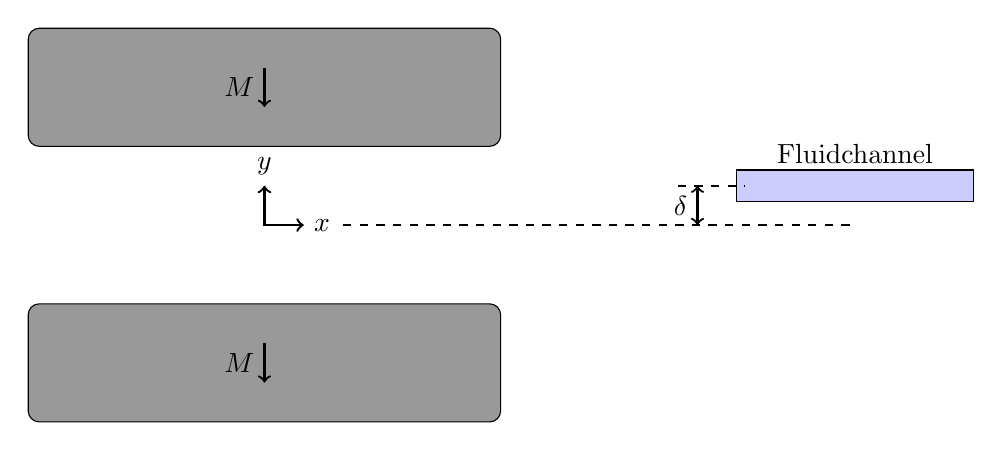
\begin{tikzpicture}[scale=1]
	\filldraw[rounded corners, fill=black!40!white, draw=black] (-9,1) rectangle (-3,2.5);
	\filldraw[rounded corners, fill=black!40!white, draw=black] (-9,-1) rectangle (-3,-2.5);	
	\filldraw[fill=blue!20!white, draw=black] (0,0.3) rectangle (3,0.7);	
	\node[thick] at (1.5,0.9) {Fluidchannel};

	\draw[line width=0.3mm,<->] (-6,0.5) node[anchor=south] {$y$} -- (-6,0) -- (-5.5,0)
	 node[anchor=west] {$x$};

	\draw[thick,dashed,-] (-5,0) -- (1.5,0);
	\draw[thick,dashed,-] (-0.75,0.5) -- (0.1,0.5);
	\draw[thick,<->] (-0.5,0) -- node[thick,anchor=east]{$\delta$} (-0.5,0.5);
	\draw[thick,->] (-6,2) -- node[thick,anchor=east]{$M$} (-6,1.5);
	\draw[thick,->] (-6,-1.5) -- node[thick,anchor=east]{$M$} (-6,-2);
\end{tikzpicture}
\caption[Schematic of vertical misalignment of the fluid channel]{Schematic of vertical misalignment of the fluid channel from its central plane ($y=0$) position. The parameter $\delta$ determines the distance by how much the fluidic channel has been misplaced out of centre.}%
\label{fig:doubleMagnetConfigurationMisalignment}%
\end{figure}

The misalignment of the two magnets in horizontal direction, such that the two magnets have a horizontal offset relative to each other is less likely, because the magnetic attraction always aligns the two magnets automatically. Thus, a horizontal magnet misalignment will not be considered here.

A displacement $\delta$ of $100$ $\mu$m, $300$ $\mu$m and $500$ $\mu$m has been simulated, because offsets of up to $0.5$ mm were regarded as realistically possible. Since the problem no longer is symmetrical along its $x-z$ plane ($y=0$), particle trajectories were simulated across the entire cross-section of the centre inlet channel (channel 2). In order to keep the relative particle density the same as in the previous simulations, the number of simulated particles has been doubled. The starting position of the particles was kept the same for all offset values $\delta$. 

Figure~\ref{fig:relativeSeparationEfficiencyAndParticleThroughputDoubleMagnetConfigurationMagnetOffset} shows the relative separation efficiency and the particle throughput for different flow rates and different magnetic offsets.

\begin{figure}[htb]
        \centering
        \begin{subfigure}[b]{0.48\textwidth}
                \includegraphics[width=\textwidth]{img/chapters/magneticSeparation/relativeSeparationEfficiencyDoubleMagnetConfiguration_missalignment2.eps}
                \caption{}  
        \end{subfigure}
        \begin{subfigure}[b]{0.48\textwidth}
                \includegraphics[width=\textwidth]{img/chapters/magneticSeparation/throughputDoubleMagnetConfiguration_misalignment2.eps}
                \caption{}                
        \end{subfigure}
        \caption[Relative magnetic separation efficiency and particle throughput when fluidic channel has a displacement between the two magnets of the double magnet configuration]{(a) Relative magnetic separation efficiency and (b) particle throughput for flow rates ranging between $30-375$ $\mu$l/min in the main channel. The plot shows the results for a vertical magnetic displacement of $\delta=0$, $\delta=100$, $\delta=300$ and $\delta=500$ $\mu$m.}
        \label{fig:relativeSeparationEfficiencyAndParticleThroughputDoubleMagnetConfigurationMagnetOffset}
\end{figure}

The results in Figure~\ref{fig:relativeSeparationEfficiencyAndParticleThroughputDoubleMagnetConfigurationMagnetOffset} suggest that a larger misalignment $\delta$ is advantageous for the magnetic particle separation process at high flow rates ($\dot{Q} > 150$ $\mu$l/min). However, the contrary is the case at smaller flow rates ($\dot{Q} < 50$ $\mu$l/min).

This phenomena is caused by the fact that at high flow rates particles have less time to interact with the magnets, which requires a higher magnetic field to move the particles in a short period of time. A larger vertical offset, generates a larger magnetic field, because one of the two magnets will be closer and thus, has a larger attraction capability. This makes more particles to cross the critical line of $x=-0.5$ mm even when there is not much interaction time. 

%The results in Figure~\ref{fig:relativeSeparationEfficiencyAndParticleThroughputDoubleMagnetConfigurationMagnetOffset} suggest that the effect of the misalignment $\delta$ becomes more and more insignificant for higher flow rates ($\dot{Q} > 150$ $\mu$l/min). This phenomena is caused by the fact that at higher flow rates particles have not enough time to interact with the magnets, no matter how strong the magnetic force might be. Therefore, the relative particle separation efficiency and particle throughput will go towards $0 \%$ and $100 \%$, respectively.

However, at small flow rates ($\dot{Q} < 100$ $\mu$l/min) the effect of the misalignment can no longer be neglected. It is interesting to see that at small flow rates the relative separation efficiency is not a monotonic decreasing function with respect to the parameter $\delta$. Due to the non-linearities of the magnetic force different offset values $\delta$ result in different relative separation efficiency for different flow rates. The separation efficiency is dependent on what percentage of the cross-section of the fluid channel lies above/below the $x-z$ symmetry plane. The more the fluid channel is vertically shifted away from its symmetry position (upwards or downwards), the larger the percentage of particles experience a bigger force in vertical direction. There is a trade off between the number of particles getting separated and the number of particles getting stuck. A larger offset does not necessarily result in a lower separation efficiency, because the separation efficiency is a function of the magnetic force and the particle interaction time with the magnet.

Since the separation efficiency is harder to control when the fluid channel is no longer symmetrically between the two magnets ($\delta \neq 0$), the channel was always tried to kept at $\delta=0$. Additionally the larger $\delta$, the more the setup becomes just like a single bar magnet configuration, where the gathering points for the magnetic particles will simply be at the fluid channel's inner surface which is closest to the magnet. As soon as $\delta=0.7$ mm, the gathering points no longer exist and all of the magnetic particles within a $0.4$ mm thick fluid channel will feel an attractive force towards the magnet being closest to them.

\section{Wall effects on the motion of a single particle}
\label{sec:wallEffectsOnTheMotionOfASingleParticle}
All the simulations described above suffered from particles getting stuck at the fluidchannel's inner surface. Therefore, the motion of a rigid sphere in vicinity of a wall is of great importance in this study because of the remaining vertical force of the magnetic configuration. Due to the small particle size compared to the fluid channel dimensions, the wall effect on the particle's motion of only one single plane wall is considered here. 

\begin{figure}[htb]
\centering
\begin{subfigure}[b]{0.48\textwidth}
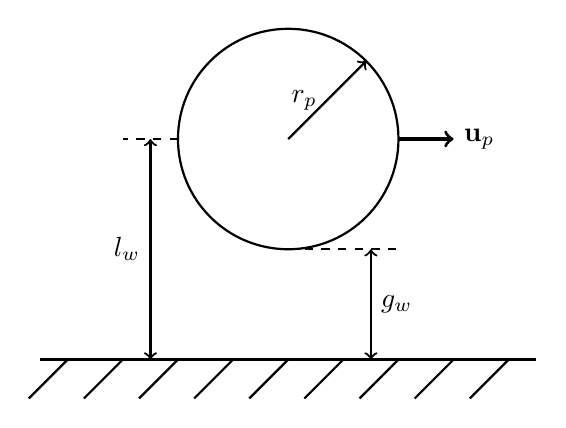
\begin{tikzpicture}[scale=0.7]
\draw[thick] (-4.5,0) -- (4.5,0);
\foreach \x in {-4,...,4} 
  \draw[thick] (\x-0.7071,-0.7071) -- (\x,0);
  
\draw[thick] (0,4) circle (2);
\draw[thick,->] (0,4) -- node[thick,anchor=east]{$r_{p}$} (1.4142,4+1.4142);
\draw[thick,dashed] (-2,4) -- (-3,4);
\draw[thick,<->] (-2.5,0) -- node[thick,anchor=east]{$l_{w}$} (-2.5,4);
\draw[thick,dashed] (0,2) -- (2,2);
\draw[thick,<->] (1.5,0) -- node[thick,anchor=west]{$g_{w}$} (1.5,2);

\draw[very thick,->] (2,4) -- (3,4) node[thick,anchor=west]{$\mathbf{u}_{p}$};
\end{tikzpicture}
\caption{} 
\end{subfigure}
%%%%%%%%%%%%%%%%%%%%%
\begin{subfigure}[b]{0.48\textwidth}
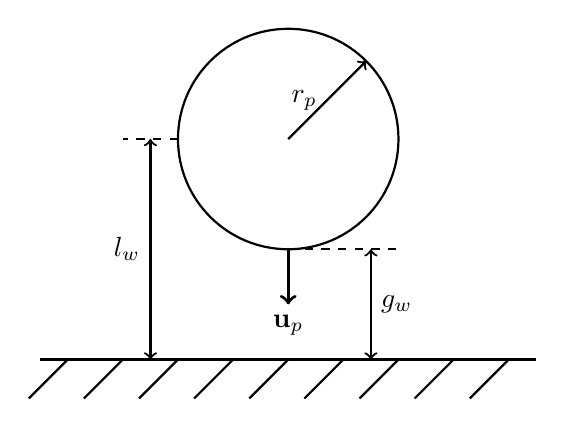
\begin{tikzpicture}[scale=0.7]
\draw[thick] (-4.5,0) -- (4.5,0);
\foreach \x in {-4,...,4} 
  \draw[thick] (\x-0.7071,-0.7071) -- (\x,0);
  
\draw[thick] (0,4) circle (2);
\draw[thick,->] (0,4) -- node[thick,anchor=east]{$r_{p}$} (1.4142,4+1.4142);
\draw[thick,dashed] (-2,4) -- (-3,4);
\draw[thick,<->] (-2.5,0) -- node[thick,anchor=east]{$l_{w}$} (-2.5,4);
\draw[thick,dashed] (0,2) -- (2,2);
\draw[thick,<->] (1.5,0) -- node[thick,anchor=west]{$g_{w}$} (1.5,2);


\draw[very thick,->] (0,2) -- (0,1) node[thick,anchor=north]{$\mathbf{u}_{p}$};
\end{tikzpicture}
\caption{} 
\end{subfigure}
\caption[Schematic of particles moving in proximity to a single plane wall]{Particles moving in proximity to a single plane wall experience different hydrodynamic forces when they move along (a) or towards (b) the wall.}
\label{fig:particleMotionCloseToWall}
\end{figure}

Particles can move either along or towards the solid wall as shown in Figure~\ref{fig:particleMotionCloseToWall}. In either case, the hydrodynamic forces on the object change when the object moves in close proximity to the wall, namely the drag force increases. In order to account for that, the drag force, initially given in Equation~\ref{eqn:dragForceOnParticle} (Chapter~\ref{ch:magnetophoresis}), needs to be adjusted by a correction factor $\beta$:

\begin{equation}
	\mathbf{F}_{D} = 6\pi\eta_{f} r_{p} \mathbf{u} \beta
	\label{eqn:wallEffectCorrectedDragForce}
\end{equation}

The two cases, given in Figure~\ref{fig:particleMotionCloseToWall}, need to be treated differently, since the correction factor $\beta$ depends on whether the particle is moving in parallel or perpendicular to the wall. Faxen worked out the influence of a single plane wall for spherical particles moving parallel to the wall~\cite{Faxen1922} and Brenner developed the model of a sphere moving towards a solid wall~\cite{Brenner1961}. Thus, the two Stokes' law correction factors for a spherical particle moving parallel ($\beta_{\parallel}$) or perpendicular ($\beta_{\perp}$) to a plane wall can be given by:

\begin{eqnarray}
	\beta_{\parallel} &=& \frac{1}{1-(9/16)(r_{p}/l_{w})+(1/8)(r_{p}/l_{w})^{3}-(45/256)(r_{p}/l_{w})^{4}-(1/16)(r_{p}/l_{w})^{5}} \\
	\beta_{\perp} &=& \frac{4}{3} \sinh(\varphi) \sum_{n=1}^{\infty} \frac{n(n+1)}{(2n-1)(2n+3)} \\
	 && \left[ \frac{2\sinh(2n+1)\alpha + (2n+1\sinh(2\alpha))}{4\sinh^{2}(n+0.5)\alpha-(2n+1)^{2}\sinh^{2}(\alpha)} -1\right] \nonumber
	\label{eqn:wallEffectCorrectionFactors}
\end{eqnarray}

where the particle radius is denoted by $r_{p}$ and the distance of its midpoint from the plane by $l_{w}$. The parameter $\varphi$ is given in terms of the ratio of sphere radius, $r_{p}$, to the distance of its centre from the plane, $l_{w}$, by the following relationship:

\begin{equation}
 	 \varphi = \cosh^{-1}(l_{w}/r_{p})
 	 \label{eqn:radiusToDistanceToPlane}
\end{equation}

Figure~\ref{fig:wallCorrectionFactors} shows the two correction factors, $\beta_{\parallel}$ and $\beta_{\perp}$, for when a spherical particle is moving at different distances away from a single wall. It can be seen that for the correction factor approaches a constant value ($\beta_{\parallel}\approx 3$) for when the particle is moving in parallel in close proximity to a wall (Figure~\ref{fig:wallCorrectionFactorsParallel}), whereas in the perpendicular case, the drag force correction factor increases infinitely (Figure~\ref{fig:wallCorrectionFactorsPerpendicular}). This means that a rigid spherical particle in a viscous fluid can never make contact with a solid surface in a finite time due to the infinite lubrication force when the distance approaches zero at the last moment of contact~\cite{Brenner1961,Cox1967,Davis1986}.% A film thickness of $1$ nm between the particle and the wall can be assumed~\cite{Lin2013}. % check this statement
s
\begin{figure}[ht]
        \centering
        \begin{subfigure}[b]{0.48\textwidth}
				\includegraphics[width=\textwidth]{img/chapters/magneticSeparation/wallDragForcCorrectionFactorParallel2.eps}
				\caption{}
				\label{fig:wallCorrectionFactorsParallel}
        \end{subfigure}                        
        %%%%%%%%%%%%%%%%
        \begin{subfigure}[b]{0.48\textwidth}
				\includegraphics[width=\textwidth]{img/chapters/magneticSeparation/wallDragForcCorrectionFactorPerpendicular2.eps}
                \caption{}
 				\label{fig:wallCorrectionFactorsPerpendicular}
        \end{subfigure}         
        \caption[Wall correction factor for spheric particles in proximity to a planar wall]{Wall correction factors for different distances from a plane surface for when a rigid spherical particle is moving (a) parallel or (b) perpendicular to the surface.}
        \label{fig:wallCorrectionFactors}
\end{figure}

Particles which are drawn towards the surface of the fluidchannel slow down in velocity because of the no slip condition of the parabolic velocity profile of the fluid. However, particles stuck to the surface do have a velocity component in $z$ direction larger than zero ($u_{z} > 0$) due to their finite size as shown in Figure~\ref{fig:particleStuckAtPlanarSurfaceVelocity}. The mean velocity of a particle which is stuck at the channel's surface can be calculated by integrating Equation~\ref{eqn:velocityProfileRectangularDuct} along the diameter of the particle. The film thickness between the particle and the wall due to lubrication force was neglected in this calculation because it is assumed to be negligible compared to the particle diameter. 
% because it makes less than $5 \%$ of the particle's radius~\cite{}. 

It could be found that the particle's mean velocity, when next to the wall, is more than $10^{2}$ times smaller than the mean fluid velocity in the fluid channel. This also means, it takes them $10^{2}$ times longer the exit the separation device, which is why particles can be assumed as \textit{lost} under continuous flow conditions.

\begin{figure}[htb]
\centering
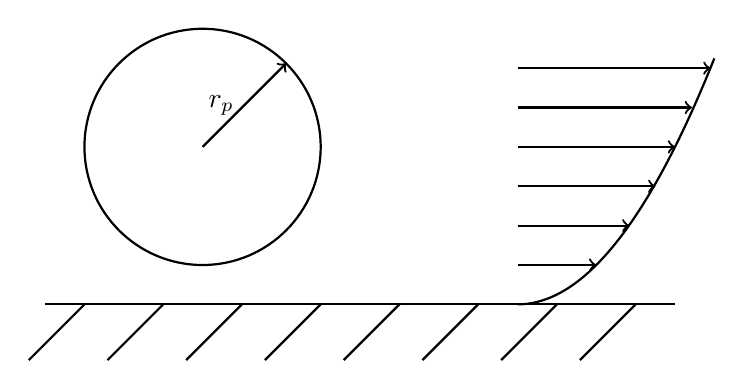
\begin{tikzpicture}[scale=1.0]
\draw[thick] (-6,0) -- (2,0);
\foreach \x in {-5.5,...,1.5} 
  \draw[thick] (\x-0.7071,-0.7071) -- (\x,0);
  
\draw[thick] (-4,2) circle (1.5);
\draw[thick,->] (-4,2) -- node[thick,anchor=east]{$r_{p}$} (-4+0.7071*1.5,2+0.7071*1.5);

\draw[thick,scale=1,domain=0:2.5,smooth,variable=\x] plot ({\x},{0.5*\x*\x});
\draw[thick,->] (0,0.5) -- (1.0,0.5);
\draw[thick,->] (0,1.0) -- (1.42,1.0);
\draw[thick,->] (0,1.5) -- (1.75,1.5);
\draw[thick,->] (0,2.0) -- (2.0,2.0);
\draw[thick,->] (0,2.5) -- (2.215,2.5);
\draw[thick,->] (0,3.0) -- (2.45,3.0);
\end{tikzpicture}
\caption[Schematic of spherical particle in a flow field in proximity to a planar wall]{A spherical particle in a flow field in close proximity to a planar will still experience a certain drag force due to its finite size.}
\label{fig:particleStuckAtPlanarSurfaceVelocity}
\end{figure}

However, it could be experimentally shown, that particles can be moved even if they got stuck at the surface. If a flow rate of $10$ ml/min or higher is used, particles and particle agglomerates could be successfully flushed out of the system. Theoretically, flow rates of up to $112$ the ml/min still remain in the laminar flow regime in fluid channel since the Reynolds number stays below its critical value of $\text{Re} \approx 2100$. This means, particles are not flushed out of the system because of eddies caused by turbulences, but are rather pushed because of the drag force they experience. At a flow rate of $10$ ml/min particles attached to the surface experience a mean velocity of $1.2$ mm/s. The drawback of such high flow rates is that the majority of particles will have such a short magnet interaction time such that they will pass straight through the separation device without even \textit{noting} the magnet.

The fact that there is always a factor of $10^{2}$ between the average particle velocity across the channel and the particles in contact with the wall makes it extremely difficult for continuous separation to be efficient. A pulse mode, where particles are gathered and flushed in alternating cycles seems to be a more promising alternative. 

\section{Particle trajectory simulation in pulse mode}
\label{sec:pulseModeParticleSeparationSimulation}
Particles which are attached to a surface are regarded as stuck due to their slow moving velocity. However, even if particles on the surface no longer experience sufficient drag to move along the channel ($z$ direction), they are still exposed to the magnetic field. This means they are still moving perpendicular to the fluid flow due to magnetophoresis. Their movement in horizontal direction ($x-z$ plane) along a wall will be slower by a factor of $\beta_{\parallel} \approx 3$ than in free flow because of the increasing drag force, as seen above (Figure~\ref{fig:wallCorrectionFactorsParallel}). 

This property can be used in the magnet particle separation, double magnet as well as quadrupole magnet configuration, when run in pulse mode. The idea behind is, that the fluid channel first gets filled with particle laden fluid. The fluid flow is then significantly reduced or completely switched off, leaving the particles time to move to the gathering positions. Once all the particles have reached their stable gathering positions, the particles are then flushed out of the magnetic separation device using a high flow rate again. Thereby, the flushing flow rate was kept in the laminar regime, where it can be assumed that no turbulences occur and that all particles still follow their streamlines perfectly.

However, the ideal time cycle between particle gathering ($|\dot{Q}| \approx 0$) and particle flushing ($|\dot{Q}| >> 0$) needs to be determined. Therefore, particle trajectories for different time intervals at different positions along the $z$ axis have been simulated. The flow rate is set to $\dot{Q}=0$ and the particle-wall model described in Section~\ref{sec:wallEffectsOnTheMotionOfASingleParticle} is incorporated in the simulation. 

In this analysis a quadrupole magnet configuration (Figure~\ref{fig:quadrupoleMagnetConfiguration}) was assumed with a vertical and a horizontal gap between the magnets of $a=2.64$ mm and $b=3.5$ mm, respectively. When using the quadrupole magnet configuration, where the gathering points are on the vertical centre plane ($y-z$ plane), magnetic particles were introduced through the sheath flows (inlet 1 and inlet 3), and separated from the sample flow into channel 2. Due to the additional symmetry of this configuration, only one quarter was simulated, as depicted in Figure~\ref{fig:particleIntroductionSchemeDoubleMagnetConfigurationQuadrupole}. 

\begin{figure}[htb]
        \centering
        \begin{subfigure}[b]{0.45\textwidth}
                \includegraphics[width=\textwidth]{img/chapters/magneticSeparation/particleInletHydrodynamicFocusingSchemeQuadrupole.PNG}
                \caption{}  
        \end{subfigure}
        \begin{subfigure}[b]{0.45\textwidth}
                \includegraphics[width=\textwidth]{img/chapters/magneticSeparation/particleInletCrosssectionSchemeQuadrupole.PNG}
                \caption{}                
        \end{subfigure}
        \caption[Schematic where particle are introduced in the pulse mode simulation]{Schematic where particle are introduced in the pulse mode simulation. The grey area indicates particle laden solution. (a) Top view: Particles are released through the center channel of the separation device. (b) Cross sectional view: Particles are randomly distributed across the top half of the center channel due to symmetry. Sketches are not to scale.}
        \label{fig:particleIntroductionSchemeDoubleMagnetConfigurationQuadrupole}
\end{figure}

Figure~\ref{fig:separationEfficiencyQuadrupoleMagnetConfigurationPulseMode} shows the relative separation efficiency at different positions along $z$ for various time intervals $\Delta\text{t}$. The throughput is deliberately not shown here, because it is assumed that all particles can be recovered when flushing. Therefore, the relative separation efficiency is also the absolute efficiency in this case.

\begin{figure}[htb]
\centering
\includegraphics[width=0.7\textwidth]{img/chapters/magneticSeparation/separationEfficiencyQuadrupoleMagnetConfigurationPulseAlongZ.eps}
\caption[Separation efficiency of quadruple magnet configuration in pulse mode]{Separation efficiency of the quadruple magnet configuration in pulse mode along different $z$ slices. The separation simulation was calculated at steady flow conditions ($\dot{Q}=0$). Only half  of the fluid channel ($z \geq 0$) needed to be simulated due to symmetry. The dashed vertical line indicates the magnet edge.}
\label{fig:separationEfficiencyQuadrupoleMagnetConfigurationPulseMode}
\end{figure}

The simulation makes it obvious that the larger $\Delta\text{t}$, the more likely all particles reach their stable gathering points, which improves the separation efficiency. This is only true for particles released within the \textit{impact zone} ($-10 \text{mm} < z < 10 \text{mm}$) of the magnet configurations. However, even within the magnetic impact zone the time needed to remain the level of separation efficiency increases when moving away from the origin ($x=y=z=0$) in $z$ direction because the magnetic field becomes weaker. Outside of the impact zone the unique magnetic field decays quickly and its gathering points vanish. This means particles might still be effected by the applied magnetic field but are no longer moving towards specific points or it takes them too long to do so. Thus, these particles will not be efficiently separated even after $\Delta \text{T}$ approaches infinity ($\Delta \text{t} \rightarrow \infty$), which reduces separation efficiency.

%The quadrupole configuration suffers from the same limitation like the double magnet configuration. The overall separation time could be reduced due to higher magnetic driving forces, but particles outside of the magnetic impact zone are not getting efficiently separated again, as shown in Figure~\ref{fig:scatterPlotQuadrupoleMagnetConfigurationPulseMode}.

%\begin{figure}[htb]
%\centering
%\begin{tikzpicture}[scale=1.0]
%	\draw (-2,-2) rectangle (2,2);
%\end{tikzpicture}
%\label{fig:scatterPlotQuadrupoleMagnetConfigurationPulseMode}
%\caption[]{Separation efficiency of the quadruple magnet configuration in pulse mode along different $z$ slices. The separation simulation was calculated at steady flow conditions ($\dot{Q}=0$). Only one eight of the fluid channel needed to be simulated due to symmetries in the magnet geometry. The dashed vertical line indicates the magnet edge.}
%\end{figure}

Unfortunately, these findings propose that a separation efficiency of $100\%$ can never be achieved with the current configuration geometries, even when run in pulse mode. Because when the magnetic separation device is fully filled with particle laden fluid, there will always be some \textit{spillage} of the particles because they do not initially start within or in close proximity to the magnetic impact zone. 

\section{Continuous particle separation experiment}\label{sec:continuousParticleSeparationExperiment}
To demonstrate the separation efficiency of magnetic particles from the sample inlet, a mixture of $1$ $\mu$m sized magnetic particles (Chemicell) and blue non-magnetic silicon beads of $0.4$ $\mu$m in diameter were used. The particle sample was prepared by diluting the magnetic particles with deionised (DI) water to a concentration of $10^{6}$ particles/ml and then adding the blue silicon beads. The concentration of the blue beads was chosen such that the sample liquid was died blue to enable the hydrodynamic focusing to be viewed clearly.

The surfactant Pluronic F-127 (Sigma-Aldrich) at $0.01 \%$ weight to volume ratio was added to the particle suspension to prevent adhesion of particles to the fluidchannel surfaces and also a mixture of DI water and $0.1 \%$ of F-127 was used to flush the fluidic channel for $5$ min prior to each experiment. The two sheath flows, used to focus the magnetic particle containing sample flow, was also a mixture of DI water and $0.1 \%$ of F-127.

The microfluidic device was connected to three $1$ ml glass syringes (BD Biosciences, UK) mounted on Harvard syringe pumps using $0.5$ mm inner diameter flexible tubing to introduce the flows to the device. The inlet channels of the microfluidic device were visualised and data recorded using a CCD camera mounted on an inverted microscope. The outlet channels were connected by the same tubing to three $0.5$ ml collection pots (Microfluidic Chip Shop, Germany) mounted on the fluid device, which were capped after each experiment and removed for further analysis. 

In order to achieve steady state, the experiment was allowed to run for five minutes. The hydrodynamic focusing was adjusted in each of the three inlet flows in order to fill, but not overspill, their respective exit channel, when conducting the separation experiments. Thereby, the aspect ratio of the flow rates between the channel inlets was kept as close to $1$, whilst maintaining the hydrodynamic focusing.  

The magnetic particles entering the device through the centre channel (channel 2) were pulled through magnetophoresis from the hydrodynamically focused sample flow towards their gathering points, where the particles no longer experience a horizontal force. A clear separation was visible as seen in Figure~\ref{fig:doubleMagnetSeparationExperiment}.

\begin{figure}[htb]
   \centering
   \includegraphics[width=0.7\textwidth]{img/chapters/magneticSeparation/doubleMagnetSeparationExperiment.jpg}
   \caption[Double magnet particle separation experiment in continuous flow]{The separation of magnetic particles (orange) from a mixture of magnetic particles and blue non-magnetic beads achieved in continuous flow using the double magnet configuration.}
   \label{fig:doubleMagnetSeparationExperiment}
\end{figure}

Visual observations showed that magnetic particles were continuously deflected by the magnet from the central sample flow into the buffer flow which suggested that separation of magnetic particles was achieved. 

The relative separation efficiency of the separation setup was then determined by analysing the collected outlet samples using flow cytometry (BD Accuri C6). Measuring the samples at the three outlet channels by flow cytometry indicated that the majority of magnetic particles ($>65\%$) were not deflected by the magnets and travelled straight through the device along their streamlines as depicted in Figure~\ref{fig:relativeSeparationEfficiencyContineousExperimentDoubleConfiguration}. This shows that most particles did not have enough time to interact with the magnetic field to be drawn from the sample into the butter flow.

\begin{figure}[htb]
   \centering
   \includegraphics[width=0.7\textwidth]{img/chapters/magneticSeparation/relativeSeparationEfficiencyExperiment.eps}
   \caption[Particle separation efficiency of the double magnet configuration in continuous flow]{Relative separation efficiency for different flow rates in the main channel. The experiment has been repeated $3$ times for the shown flow rates.}
   \label{fig:relativeSeparationEfficiencyContineousExperimentDoubleConfiguration}
\end{figure}

Further examination using higher resolution microscopy revealed that what was observed by eye as magnetically separated particles were in fact particles which became \textit{stuck} at the top or the bottom due to vertical magnetic forces. These particles were slowly rolling along the channel's inner surface because of the no slip boundary condition of the fluid and were forming large agglomerates.

%The separation results for the double magnet configuration, however, were surprisingly  high compared to the simulated results for the used flow rates, but at the same time low compared to the visual inspection. 

%As expected from the numerical simulations, the separation efficiency of the double magnet configuration was found to be negatively correlated to the total flow rate in the microfluidic separation device. 

\section{Particle separation experiment in pulse mode}\label{sec:particleSeparationExperimentInPulseMode}
The quadrupole configuration was more efficient at focussing the magnetic particles away from the sample stream and into the channel for separation. Although there was a definite sideways migration of the particles into the central stream, they also experienced an upwards acting force, causing them to agglomerate at the surfaces of the device. A continuous separation efficiency of only $55\%$ could be achieved in the experiments (Figure~\ref{fig:separationEfficiencyPulseExperimentQuadrupoleConfiguration}). It was again observed that separation under continuous flow did not allow enough time for all magnetic microparticles to migrate into the central exit channel. Many were still found in the introductory exit channel. To improve this separation, the quadrupole configuration was run in a pulse mode.

A strategy of introducing magnetic particles for 30 seconds, then pausing all flows for $60$ seconds and repeating this for ten cycles, before using a fast flush of $1000$ $\mu$l/ min for $10$ seconds, was used to increase the residence time of the magnetic particles in order for them to migrate into the designated region and to be separated. Nearly $90\%$ of the magnetic microparticles were separated from the sample flow when using the quadrupole magnet configuration in pulse mode, as shown in Figure~\ref{fig:separationEfficiencyPulseExperimentQuadrupoleConfiguration}. Figure~\ref{fig:separationEfficiencyPulseExperimentQuadrupoleConfiguration} also shows the continuous separation efficiency ($56\%$) when run with $36$ $\mu$l/min for comparison.

\begin{figure}[htb]
\centering
\includegraphics[width=0.7\textwidth]{img/chapters/magneticSeparation/relativeSeparationEfficiencyExperimentQuadrupole.eps}
\caption[Particle separation efficiency of the quadrupole configuration in pulse mode]{The separation efficiency of the quadrupole configuration in continuous and pulsed mode compared to the control when no magnets is present. A flow rate of $36$ $\mu$l/min was used in the continuous mode.}
\label{fig:separationEfficiencyPulseExperimentQuadrupoleConfiguration}
\end{figure}

Unfortunately, the experiment was not exactly done in the same manner as the simulation. But an average interaction time between the particles and the magnet of approximately $500$ seconds can be assumed for the experiment. The simulation showed almost $100\%$ separation a long the entire length of the fluid channel. In order to work out the separation efficiency of the simulation when the channel gets flushed one has to integrate the values along $z$. However, the exact function is unknown and therefore only an approximation can be given. 
 

\section{Discussion and Conclusion}\label{sec:discussionAndConclusionMagneticSeparation}
The separation efficiency for continuous flow of a double magnet configuration as well as for pulse flow in a quadrupole magnetic configuration has been investigated. The novel magnet configurations were designed to remove or concentrate magnetic particles from a sample solution.

Low magnification viewing of the separation indicated a good separation of the magnetic particles when using the double magnet configuration setup. However, analysis by flow cytometry highlighted that, at the flow rates used, many particles passed through the device without being deflected from the sample flow. Another large percentage of particles are getting stuck at the inner surface of the microfluidic device. The same findings were also made by the simulations. However, the simulation results suggested a lower relative separation efficiency than what was measured in the experiments. The discrepancy between the experiment and the simulation was tried to be explained by simulating possible scenarios such as different particle mobilities, particle agglomeration or misalignment of the microfluidic channel. The experimental results could not be matched in any of the continuous separation simulations. This indicates that other forces, which are not included in the model, must play a role. It could be seen in the experiments that particles gathered at the surface of the fluid device have a tendency to attract other particles and then form large clusters, which occasionally break off when they become large enough. These particle-particle interaction forces are not modelled in the simulation, but contribute positively to the separation efficiency in the experiments. 

Despite the hydrodynamic focusing, magnetic particles are introduced at different positions across the sample inlet's cross section and were therefore subjected to different forces and moving distances. These differences are responsible for the trapping and \textit{loss} of particles in the fluidic device. This also caused a unique particle introduction pattern for every continuous flow rate used from where particles needed to be introduced into the system in order to get effectively separated. If a more localised introduction of the magnetic particles could be found, the predictability of the trajectories and thus the separation efficiency could be increased. In order to launch particles more accurately a 3D hydrodynamic focusing should be considered, how it is used in flow cytometry or described by Zborowski \etal~\cite{Zborowski2011a}. Also reducing the dimensions of the device, particularly its width, might help mitigate this problem because particles no longer have to move over such a wide distance to be regarded as separated.

In order to recover all the injected magnetic particles a pulse mode is introduced, where fast and slow flow rates alternate, while using a magnetic quadrupole configuration. When operating in pulsed mode high separation efficiency could be achieved in the simulation as well as in the experiments. The simulation showed that an increase in the pause time (slow flow rate) positively effected the absolute separation, since it allows an longer residence time for the particles to migrate to the gathering points. 

The simulation also showed the practical limitation of the quadrupole configuration, because the unique magnetic field decays when at a distance away from the setup. Particles out side of the magnetic impact zone experience a much weaker magnetic force. Therefore, their time needed to move to their gathering points can take infinitely long. By shaping or tapering the magnets at the ends one could alter the magnetic flux to have the unique separating magnetic field along the entire length of the microfluidic device.  

Even if Chapter~\ref{ch:magnetophoresis} has shown that a constant mobility can only be taken as an approximation for the applied magnetic field strength used here, the simulations performed in this chapter should still be significant because a difference in mobility only effects the time needed for the particle to move to its designated position. In the case of a continuous flow separation that means the initial starting position needs to be changed and in the case of a pulse mode separation, the pause time has to be increased. 

%%%%%%%%%%%%%%%%%%%%%%%%%

%Increasing the residence time of the MPs by introducing a pulsed flow regime increased the separation of MPs from the sample flow. The quadrupole configuration, when operated in a pulsed mode, was able to separate nearly $90\%$ of the MPs from the sample. % Naomi

%Additionally, it shows that the magnetophoresis mobility measurement is a promising technique to determine the susceptibility of magnetic particles. However, the technique needs further evaluation, since it still suffers from numerous potential errors, e.g. inaccurate velocity measurement or magnetic field value.

%Analysis using flow cytometry supported this observation, it was found that the majority of MPs ($>65\%$) were not deflected from the main sample flow; the MPs did not have large enough residence time within the magnetic field to be separated. It is assumed that agglomerates were separated due to their increased magnetophoretic mobility, but single MPs passed straight through the device. % naomi

%Although numerous microfluidic devices have been described [210, 236, 237], further development is required to establish higher separation efficiency whilst maintaining target cell purity [213]. The MFD incorporating magnetophoresis as described in this Chapter goes someway to improving upon previously described devices. It enables the continuous separation of MPs from a complex sample without pre-enrichment and is comparable to separation described by Xia et al, [312] where separation efficiencies are detailed as being between 50 and $90\%$.

%The separation efficiency may be improved by reducing the dimensions of the channel. The described MFD is $3$ mm in width. The MPs need to migrate at least 0.5 mm in the x direction before they are separated and can be transported in the buffer flow. When operating in the pulsed mode, an increase in the pause time will allow an increased residence time for the MPs to migrate to the ROE. This is expected to increase the separation of MPs from the sample flow. 

%The magnetic susceptibility of the MPs determines the magnetic moment and hence the force exerted upon the MPs within a magnetic field [313]. In order to increase the flexibility of the MFD, MPs with a higher magnetic susceptibility will enable the use of increased flow rates due to the increased magnetic force.



%\section{Example}
%\subsection{Particle trajectory simulation: quadrupole magnet configuration}
% particles expeience a larger repulsive force than attractive force and move more quickly to the centre. 

%\section{Result}\label{sec:results}
%As the particles enter the magnetic region in the microfluidic channel, those that are close to the top and bottom walls are immediately drawn to the walls by the strong magnetic force. Particles that enter the channel closer to the centre of the channel, far from both top and bottom walls, are directed towards the center of the channel and away from the vertical walls. When reaching the centre of the channel, the vertical component of the magnetic force pulls the particles again towards the top and bottom walls. 

%ANSYS Fluent software uses the cell-centred finite volume approach, which is the most widely used, and which solves conservation equations directly at the cell centres, and uses interpolation to express the variables values $\Sigma$ at the element centroid in terms of the nodal values at the CV surface. 

%\section{Examples}
%Furthermore, the density of the particles $\rho_{p}$ is assumed to be much higher than the density of fluid so that the dominant force on an individual particle is the Stokes drag. 

%Nowadays, due to the dramatic progress in the quality and speed of computers, the simulations can be reasonably performed on workstations. 

%In an automated process, such as in a clinical diagnostic instrument, the length of time required for complete separation may become a limiting factor in instrument throughput. A modelling process with the goal of optimizing magnet and cuvette design is therefore useful for maximizing instrument performance.  

%%%%%%%%%%%%%%%%
%Various different designs for HGMS have been published in the past. A new design is presented here, which offers the advantage to separate particles independently of their magnetophoretic mobility while reducing particle wall interaction. 

%%%%%%%%%%%%%%%
%An important characteristic of the fluidic dynamics is the parabolic flow through a rectangular channel and the resultant zero velocity at the internal surfaces of the channel. This flow regime is well documented  in rectangular fluid channels $[309]$. When MPs hit a surface of the device, there will be zero velocity to drive the MPs along and out of the MFD. MPs will be deemed as lost if they arrive at an internal surface, as they are difficult to recover using continuous flow at low flow rates. In order for surface collisions to be minimised, and therefore the number of lost MPs, careful design of the magnetic field is necessary.  % Naomi

%%%%%%%%%%%%%%%
%As mentioned in chapter 2, conventional particle simulation approaches are based on the point-particle approximation.


%%%%%%%%%%%%%%%%%%
%There are two types of magnetophoretic microfluidic separation device: batch and continuous. Batch separation involves the trapping of MPs by an external magnet, the removal of the supernatant and the capture of the trapped particles once the magnetic field has been removed. Continuous methods [299] have been described, however, these methods present certain difficulties. The agglomeration of MPs is a particular problem. The greater the number of particles within close proximity of each other, the greater the magnetic force acting upon them due to their induced magnetic dipoles. This encourages particle agglomeration [300] which results in differing mobilities and velocities in the gradient magnetic field [301]. Even at low concentrations of MPs, variations in their physical properties cause undesirable differing mobilities, that can lead to poor separation efficiency. To overcome this problem, novel magnet configurations were devised with the aim of using MPs of any size, susceptibility and concentration, to be continuously separated from a sample using microfluidics (Figure 4.1). The MPs are encouraged into a (ROE) where no magnetic force is experienced by the MPs; subsequently the MPs are separated by a continuous, hydrodynamically-focussed buffer flow. % Naomi

%%%%%%%%%%
%The scatter plots in Figure~\ref{fig:scatterPlotDoubleMagnetConfigurationPulseMode} show the starting and end points of the particles after different finite gathering time steps released at various $z$ slice for the double magnet configuration. It becomes evident again that particles released at a distance $|z| > 11 \text{mm}$ do no longer interact with the magnets enough, to have a high separation efficiency guaranteed. 
%
%\begin{figure}[htb]
%\centering
%\begin{tikzpicture}[scale=1.0]
%	\draw (-2,-2) rectangle (2,2);
%\end{tikzpicture}
%\caption[]{Scatter plot of the particle position after multiple time intervals $\Delta\text{T}$ when a double magnet configuration is used.}
%\label{fig:scatterPlotDoubleMagnetConfigurationPulseMode}
%\end{figure}
